\chapter{Parameters Update}

IMPORTANT NOTATION!!: Through all this chapter I am saying parameters = weights, but remember that there are other ones like the bias.

\section*{First Order Optimization Methods}
The pseudo-code for updating the parameters:
\begin{lstlisting}[frame=single]
while True:
     data_batch = dataset.sample_data_batch()
     loss = network.forward(data_batch)
     dw = network.backward()
     w += -learning_rate * dw
\end{lstlisting}

This update (\texttt{w+=-lr*dw}) is an stochastic gradient descent. Let's see better ways of updating the parameters. The plot below shows different update strategies to optimize the loss function. In DNN, as you scale your model, local minima become less and less of an issue. The loss function shape we should have in mind is like a landskape with a lot of local minima but all with more or less the same loss. As you scale the model the distance between the bigger and lower local minima scales down (there is no bad local minima in big networks).

\subsection*{Stochastic gradient descent}
\begin{equation}
w_t = w_{t-1} -\alpha \bigtriangleup L(w_{t-1})
\end{equation}

where $\bigtriangleup L(w_{t-1})$ is the derivative of the loss function and  the learning rate

\begin{figure}[h]
  \centering
  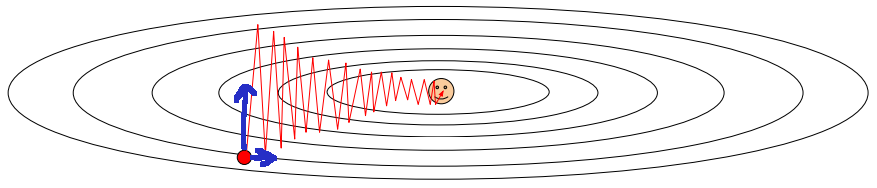
\includegraphics[width=0.6\textwidth]{Images/params_up/1.png}
  \caption{SGD example}
\end{figure}

\textbf{Problem:}
Supose a 2dimensions loss function (NN with 2 layers and 2 weights) which is steep vertically and shallow horizontally (weight represented in the vertical axis has a higher impact over the loss function). The horizontal gradient is small because it is a shallow function in the horizontal direction, and a big gradient in the vertical direction because it is steep in this direction. Then, the update is way too slow in the horizontal direction, and to fast in the vertical direction. This causes an ugly jerk shape.

Notice that it is not an option to just decrease the learning rate because then it would take forever to cross all the shallow surface.

IMPORTANT NOTATION!!: Through all this chapter I am saying parameters = weights, but remember that there are other ones like the bias.

\subsection*{Momentum update}
\begin{equation}
\begin{aligned}
v_0 &= 0 \\
v_t &= \mu v_{t-1} - \alpha \bigtriangleup L(w_{t-1}) \\
w_t &= w_{t-1} + v_t
\end{aligned}
\end{equation}

where $\mu \in [0,1]$ and usually takes values around ~0.5, ~0.9 or 0.99 (sometimes annealed over time 0.5 -> 0.99)

It can be interpreted as a ball rolling across the loss function starting at velocity 0. Notice that  would represent position,  velocity,  friction (decreasing velocity over time). Now you will speed up in shallow surfaces directions and in steep directions you will be jiggly but you will have a force pushing you to the center (like a ball rolling in a convex function).


In the first plot we can see that first it overshoots because of all the accumulated velocity but it ends converging to the minimum quicker than SVG.

\subsection*{Nesterov Momentum update (or Nesterov accelerated gradient descent) }
\begin{equation}
\begin{aligned}
v_0 &= 0 \\
v_t &= \mu v_{t-1} - \alpha \bigtriangleup L(w_{t-1} + \mu v_{t-1}) \\
w_t &= w_{t-1} + v_t
\end{aligned}
\end{equation}
A slightly different version of the momentum update has recently been gaining popularity. It enjoys stronger theoretical converge guarantees for convex functions and in practice it also consistenly works slightly better than standard momentum.

The core idea behind Nesterov momentum is that when the current parameter vector is at some position $x$ (weights), then looking at the momentum update above, we know that the momentum term alone (i.e. ignoring the second term with the gradient) is about to nudge the parameter vector by $\mu * v$. Therefore, if we are about to compute the gradient, we can treat the future approximate position $x + \mu * v$ as a “lookahead” - this is a point in the vicinity of where we are soon going to end up. Hence, it makes sense to compute the gradient at $x + \mu * v$ instead of at the “old/stale” position $x$.

\begin{figure}[h]
  \centering
  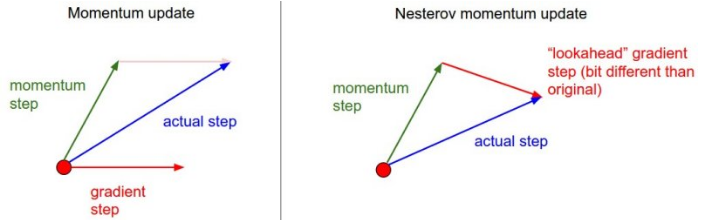
\includegraphics[width=0.7\textwidth]{Images/params_up/2.png}
  \caption{Nesterov Momentum update}
\end{figure}

IMPORTANT NOTATION!!: Through all this chapter I am saying parameters = weights, but remember that there are other ones like the bias.

\subsection*{AdaGrad} 
\begin{equation}
\begin{aligned}
c_t &= c_{t-1} + \bigtriangleup L(w_{t-1})^2 \\
w_t &= w_{t-1} - \frac{\alpha  \bigtriangleup L(w_{t-1})}{\sqrt{c_t} + 1^{-7}}
\end{aligned}
\end{equation}

where  is the cache is a giant vector of the same size of your parameter vector . So this cache keeps track of the sum of squares (or also called the uncentered second moment) of your parameters in each direction (array). So now, with the cache, each dimension of the parameter vector has a different dynamic learning rate which is dynamically scaled based on what kind of gradients are you seeing in terms of their scale.

In the first case explained steep vertically and shallow horizontally loss function (2 weights). We have a large gradient vertically which will be added to cache. So in the vertical direction, the parameter update will be getting smaller and smaller (= smaller steps) because the denominator keeps increasing (= learning rate keeps decreasing). In the horizontal direction the surface is shallow, so  will be small and as a consequence the learning rate will not decrease.  The horizontal direction will have faster progress relative to the vertical direction.

So the cache is acting as an equalizer accounting for the stiffness ( ) of the loss function in the parameters direction. Keep in mind that this equalizer effect over a specific parameter (=weight) is independent of the rest of parameters. It is not like a normalization.

Problem: When training over long time the step size (= learning rate) goes to 0 and the network stops learning. To solve this, the next method is proposed.

\subsection*{RMSProp}
\begin{equation}
\begin{aligned}
c_t &= \gamma c_{t-1} + (1-\gamma) \bigtriangleup L(w_{t-1})^2 \\
w_t &= w_{t-1} - \frac{\alpha  \bigtriangleup L(w_{t-1})}{\sqrt{c} + 1^{-7}}
\end{aligned}
\end{equation}
The idea is that instead of keeping the sum of squares in every direction of the parameters, we make the counter leaky by introducing the decay rate . So we maintain the nice effect of equalizing the directions but it will not converge to 0. The term  is there just to prevent the division by 0.

You can also imagine the decay rate as a sort of a forgetting factor that makes the cache  only a function of the last few gradient but in an exponential weighted sum rate. Also, notice that we could not do something like having a sliding window just to track the previous n gradients because it would take too much memory.

Comparing RMSProp vs AdaGrad in DNNs, in practice AdaGrad usually ends up stopping too early.

IMPORTANT NOTATION!!: Through all this chapter I am saying parameters = weights, but remember that there are other ones like the bias.

\subsection*{Adam update - USE THIS ONE}
\begin{equation}
\begin{aligned}
v_0 = c_0 = 0
v_t = \frac{\mu v_{t-1} + (1-\mu)\bigtriangleup L (w_{t-1})}{1 - \mu^t} \\
c_t = \frac{\gamma c_{t-1} + (1-\gamma)\bigtriangleup L (w_{t-1})^2}{1 - \gamma^t} \\
w_t &= w_{t-1} - \frac{\alpha v_t}{\sqrt{c} + 1^{-7}}
\end{aligned}
\end{equation}
Adam update is a combination of adaptive scaling (AdaGrad) and momentum (Momentum update).  is the velocity and  the cache. Sometimes  and   are detonated first and second momentum, respectively. To compensate the fact that the momentums are initialized to zero () and need some time to "warm up", we introduce a bias correction in order to scale up  and  in the first iterations so you do not get a very biased estimate of the first and second momentum.
bias correction: $ \frac{1}{1 - \mu^t}, \frac{1}{1 - \gamma^t},$


So in DNNs you are in a stochastic setting, you are sampling from a mini-batch, there is going to be a lot of randomness in the forward pass. In other words, you are getting a lot of noisy gradients.

\begin{itemize}
\item Momentum contribution: So instead of using every gradient at every single time step we only use the decaying sum of previous gradients which helps use stabilize your gradient direction a bit.
\item Cache contribution: To make sure that  the steps size workout in steep and shallow directions.
\end{itemize}

Usually $\mu = 0.9, \gamma = 0.995$ but if you cross-validate them it can help a bit.

Why using momentum update instead of Nesterov Momentum update? It could be also done but it does not make such a difference.

IMPORTANT NOTATION!!: Through all this chapter I am saying parameters = weights, but remember that there are other ones like the bias.


\subsection*{Learning Rate - Decay over time}

So which is the best learning rate for training DNNs?
None. The best one is to start with high learning first because it optimizes faster than the "good learning rate", in this way you do really fast progress. But at some point you are going to be too stochastic and you can not converge to a minimum. So, at this point you must start decreasing the learning rate.

\begin{figure}[h]
  \centering
  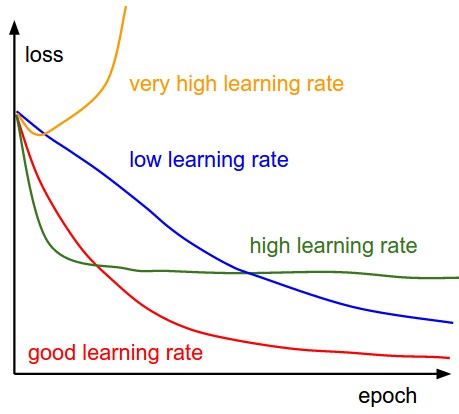
\includegraphics[width=0.35\textwidth]{Images/params_up/3.jpeg}
  \caption{Learning rate selection}
\end{figure}

Another way of seeing it is to have in mind is that with a high learning rate, the system contains too much kinetic energy and the parameter vector bounces around chaotically, unable to settle down into deeper, but narrower parts of the loss function.

 Knowing when to decay the learning rate can be tricky: Decay it slowly and you’ll be wasting computation bouncing around chaotically with little improvement for a long time. But decay it too aggressively and the system will cool too quickly, unable to reach the best position it can. There are three common types of implementing the learning rate decay:

\begin{itemize}
\item \textbf{Step decay}: Reduce the learning rate by some factor every few epochs. Typical values might be reducing the learning rate by a half every 5 epochs, or by 0.1 every 20 epochs. These numbers depend heavily on the type of problem and the model. One heuristic you may see in practice is to watch the validation error while training with a fixed learning rate, and reduce the learning rate by a constant (e.g. 0.5) whenever the validation error stops improving.
\item \textbf{Exponential decay} has the mathematical form $\alpha = \alpha_0 e^{-kt}$, where $\alpha_0, k$ are hyperparameters and  is the iteration number (but you can also use units of epochs).
\item \textbf{1/t decay} has the mathematical form $\alpha = \frac{\alpha_0}{1+Kt}$ where $\alpha_0, k$ are hyperparameters and is the iteration number.
\end{itemize}


In practice, we find that the step decay dropout is slightly preferable because the hyperparameters it involves (the fraction of decay and the step timings in units of epochs) are more interpretable than the hyperparameter $k$. Lastly, if you can afford the computational budget, err on the side of slower decay and train for a longer time.

Notice that Adagrad, RMSProp and Adam already have a learning decay. When using this methods it may help a little bit also adding a learning decay method. For SGD and SGD+Momentum you should always add the learning decay.

\section*{Second Order Optimization Methods}
The advantages of second order optimization methods are: faster convergence and no hyper-parameters. However they are not normally used because they are to heavy, to much staff happening, and they use too much memory. It is preferable just to use first order methods.

The idea of second order methods is that they approximate the loss function in a more precise way. As first order methods, they approximate with an hyperplane of like which way are we sloping. Also they also approximate with Hessian (H) which is telling you how is this surface curving. So you need the gradient for the sloping estimation and the Hessian for the surface curvature.

For example in the Newton method, ones you have form this bowl like Hessian approximation to you objective function, you can use this information to jump directly to the minimum of that approximation, and you keep iterating this strategy.

\begin{equation}
\begin{aligned}
J(\theta) &\approx J(\theta_0) + (\theta - \theta_0)^T \bigtriangleup_{\theta}J(\theta_0) + \frac{1}{2}(\theta - \theta_0)^T H (\theta - \theta_0)
\theta^\ast &= \theta_0 - H^{-1}\bigtriangleup_{\theta}J(\theta_0)
\end{aligned}
\end{equation}

This method is impractical to train DNNs because it would take too much memory. So imagine you have 10 million parameters, then your Hessian matrix would of size 10 million by 10 million and then you want to invert it, so good luck.

There is a variant of the Newton method called BGFS which approximates the inverse Hessian with rank 1 over time so you do not need to compute the inverse of the Hessian but still requires to store the gigantic matrix in memory.

Another extension called L-BGFS does not require you to store all the full inverse matrix. This method is used some time to train DNNs. It usually works very good in full batch and deterministic functions with no stochastic settings. However, it does not transfer very well to mini-batch settings because the approximation it is doing of the Hessian matrix are incorrect when you switch the batch. Also, it does not work well with stochastic settings, so you have to remove all sources of randomness (e.g. dropout). Still, it is to heavy, to much staff is happening,f and it is better just to use first order methods.

\section*{Summary}
\begin{itemize}
\item Adam is a good default choice in most cases. Some times it helps adding learning rate decay like step decay or exponential decay even-though Adam already has inside a learning decay.
\item If you can afford to do full batch updates then try out L-BFGS (do not forget to disable all sources of noise/randomness)
\item Decay your learning rate over the period of the training. For example, halve the learning rate after a fixed number of epochs, or whenever the validation accuracy tops off.
\end{itemize}

IMPORTANT NOTATION!!: Through all this chapter I am saying parameters = weights, but remember that there are other ones like the bias.